% vim: set textwidth=78 autoindent:
% !TeX root = user_guide.tex

\section{Rastergel�ndeanalyse Plugin}

% when the revision of a chapter has been finalized, 
% comment out the following line:
%\updatedisclaimer

Das Rastergel�ndeanalyse Plugin erm�glicht es, Hangneigung (Neigung), 
Exposition (Perspektive), Rauhigkeitsindex und Gesamtkr�mmung auf 
Basis eines H�henmodells (DGM) zu berechnen. Es ist sehr einfach zu 
handhaben und bietet eine intuitive grafische Benutzeroberfl�che 
(siehe Abbildung \ref{fig:raster_terrain_dialog}).
Das Plugin ben�tigt die folgenden Parameter:

\begin{itemize}[label=--]
\item \textbf{Analyse}: Hier w�hlen Sie Neigung, Perspektive, 
Rauhigkeitsindex oder Gesamtkr�mmung.
\item \textbf{Eingabelayer}: W�hlen Sie eine H�hendatei aus den 
geladenen Rasterlayern aus.
\item \textbf{Ausgabelayer}: Geben Sie hier den Pfad und Namen der 
Ausgabedatei an.
\item \textbf{Ausgabeformat}: W�hlen Sie das Ausgabeformat der 
Ausgabedatei (Standard ist GeoTiff).
\end{itemize}

Der Parameter \textbf{Neigung} berechnet den Neigungswinkel f�r jedes Pixel
in Grad, basierend auf erster Ordnung oder abgeleiteter Sch�tzung. Der
Parameter \textbf{Perspektive} berechnet die Exposition f�r jedes Pixel in
Grad, beginnend mit dem Wert 0 f�r die Nordausrichtung und dann weiter gegen den
Uhrzeigersinn. Der \textbf{Rauhigkeitsindex} berechnet die quantitative
Gel�nderauhigkeit und der Parameter \textbf{Gesamtkr�mmung} 
berechnet die Kr�mmung kombinert aus vertikaler und horizontaler Kr�mmung.

\begin{figure}[ht]
   \begin{center}
   \caption{Rastergel�ndeanalyse Plugin \nixcaption}
   \label{fig:raster_terrain_dialog}\smallskip
   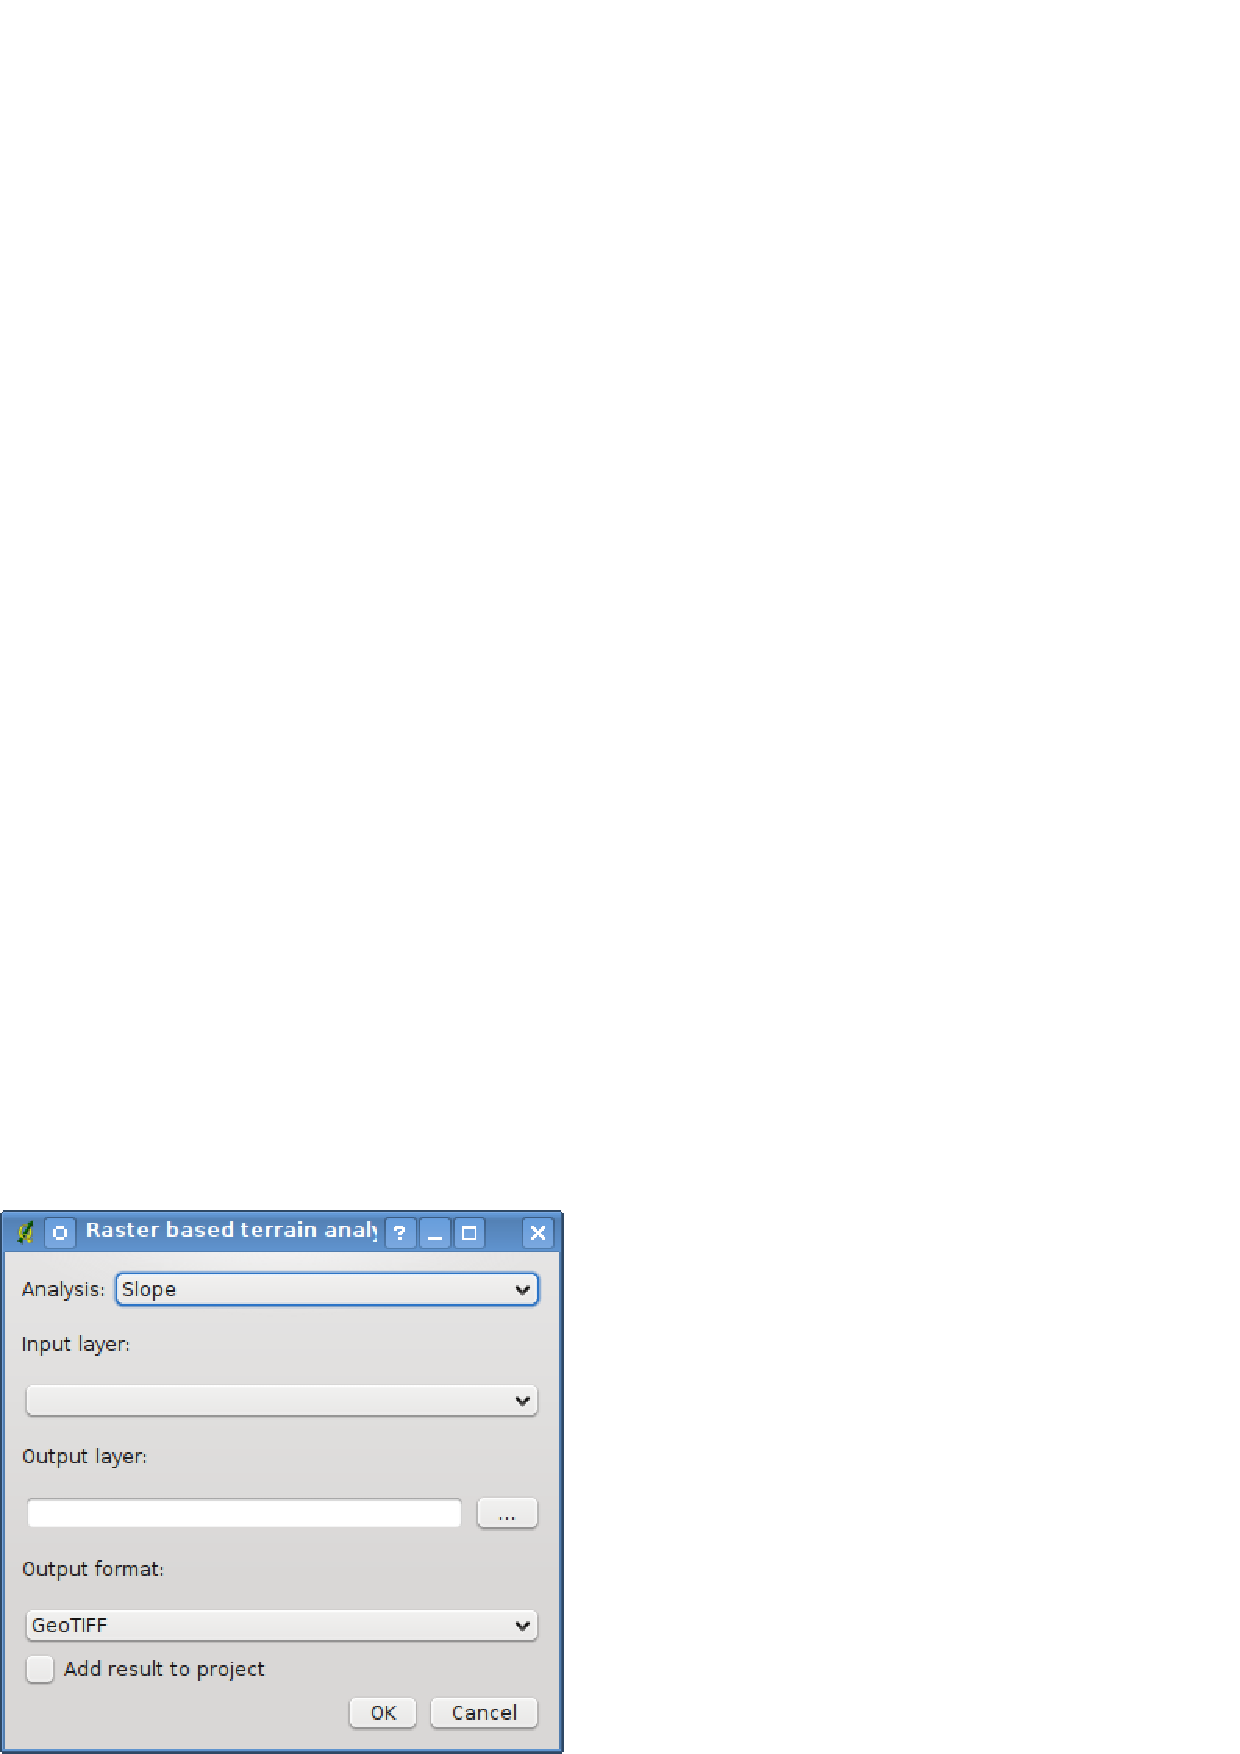
\includegraphics[clip=true, width=6cm]{raster_terrain_dialog}
\end{center}  
\end{figure}

\minisec{Das Plugin anwenden}\label{raster_terrain_usage}

\begin{enumerate}
  \item Starten Sie QGIS und laden Sie einen DGM Rasterlayer. 
  \item Laden Sie das Rastergel�ndeanalyse Plugin im Plugin Manager 
  (siehe Abschnitt \ref{sec:load_core_plugin}) und klicken Sie auf das 
  Icon \toolbtntwo{raster_terrain}{Rasterbasierende Gel�ndeanalyse} 
  in der Werkzeugleiste. Der Plugin Dialog erscheint nun, wie in Abbildung 
  \ref{fig:raster_terrain_dialog} zu sehen.
  \item W�hlen Sie eine Analysemethode (z.B.: \dropmenuopt{Neigung}).
  \item Geben Sie eine Ausgabedatei mit Pfad und Dateiformat an und 
  klicken Sie dann auf \button{Ok}.
\end{enumerate}

\FloatBarrier
